\documentclass[border=8pt]{standalone}
\usepackage[T1]{fontenc}
\usepackage{lmodern}
\usepackage{xcolor}
\usepackage{tikz}
\usetikzlibrary{shapes.geometric,arrows.meta,positioning,fit,backgrounds}
\definecolor{cLLM}{HTML}{6C5CE7}
\definecolor{cDet}{HTML}{0E9F9C}
\definecolor{cHum}{HTML}{E8963A}
\definecolor{cIn}{HTML}{64748B}
\definecolor{cAgent}{HTML}{C0392B}
\begin{document}
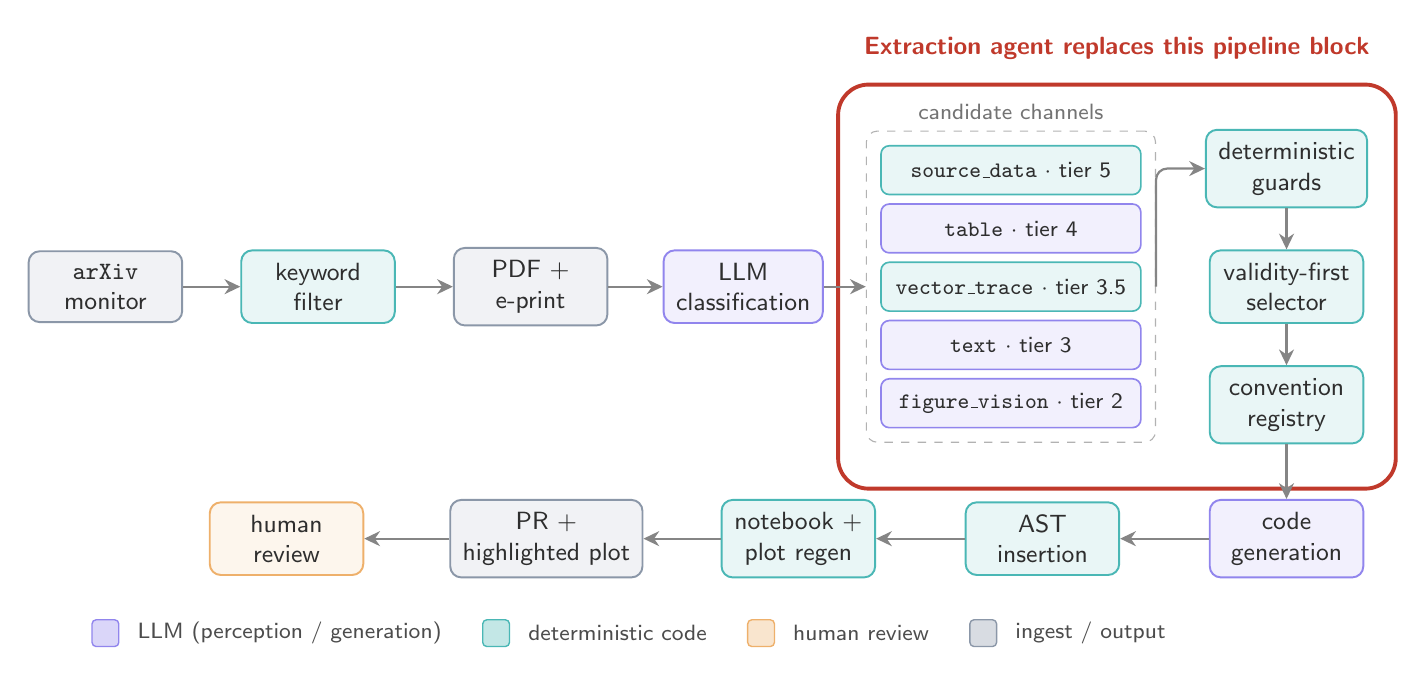
\begin{tikzpicture}[
    font=\sffamily,
    box/.style={rectangle, rounded corners=4pt, draw=#1!75, line width=0.7pt,
                fill=#1!9, text=black!82, align=center, inner sep=4.5pt,
                minimum height=0.9cm, minimum width=1.95cm, font=\sffamily\small},
    chan/.style={rectangle, rounded corners=3pt, draw=#1!75, line width=0.6pt,
                fill=#1!9, text=black!82, align=center, inner sep=3pt,
                minimum height=0.62cm, minimum width=3.3cm, font=\sffamily\footnotesize},
    flow/.style={draw=black!48, line width=0.8pt, rounded corners=4pt,
                -{Stealth[length=2mm,width=1.9mm]}},
    lgd/.style={rectangle, rounded corners=1.5pt, minimum width=0.34cm,
                minimum height=0.34cm, draw=#1!75, fill=#1!25, line width=0.5pt},
]
% discovery / ingest row  (slate = ingest, teal = deterministic, violet = LLM)
\node[box=cIn]  (arxiv) at (0,0)   {\texttt{arXiv}\\monitor};
\node[box=cDet] (kw)    at (2.7,0) {keyword\\filter};
\node[box=cIn]  (pdf)   at (5.4,0) {PDF +\\e-print};
\node[box=cLLM] (llm1)  at (8.1,0) {LLM\\classification};
% five competing channels (colour = LLM vs deterministic)
\node[chan=cDet] (csrc) at (11.5, 1.48) {\texttt{source\_data} $\cdot$ tier 5};
\node[chan=cLLM] (ctab) at (11.5, 0.74) {\texttt{table} $\cdot$ tier 4};
\node[chan=cDet] (cvec) at (11.5, 0.00) {\texttt{vector\_trace} $\cdot$ tier 3.5};
\node[chan=cLLM] (ctxt) at (11.5,-0.74) {\texttt{text} $\cdot$ tier 3};
\node[chan=cLLM] (cvis) at (11.5,-1.48) {\texttt{figure\_vision} $\cdot$ tier 2};
\begin{scope}[on background layer]
  \node[draw=black!30, dashed, rounded corners=4pt, inner sep=5pt,
        fit=(csrc)(cvis)] (chanbox) {};
\end{scope}
\node[font=\sffamily\footnotesize, text=black!55] at (11.5,2.22) {candidate channels};
% deterministic decision core
\node[box=cDet] (guards) at (15.0, 1.5)  {deterministic\\guards};
\node[box=cDet] (select) at (15.0, 0.0)  {validity-first\\selector};
\node[box=cDet] (conv)   at (15.0,-1.5)  {convention\\registry};
% integration + review, flowing right to left
\node[box=cLLM] (codegen)  at (15.0,-3.2) {code\\generation};
\node[box=cDet] (ast)      at (11.9,-3.2) {AST\\insertion};
\node[box=cDet] (notebook) at (8.8,-3.2)  {notebook +\\plot regen};
\node[box=cIn]  (pr)       at (5.6,-3.2)  {PR +\\highlighted plot};
\node[box=cHum] (human)    at (2.3,-3.2)  {human\\review};
% orthogonal flow only (horizontal / vertical, right-angle bends)
\draw[flow] (arxiv) -- (kw);
\draw[flow] (kw) -- (pdf);
\draw[flow] (pdf) -- (llm1);
\draw[flow] (llm1) -- (chanbox.west);
\draw[flow] (chanbox.east) |- (guards.west);
\draw[flow] (guards) -- (select);
\draw[flow] (select) -- (conv);
\draw[flow] (conv.south) -- (codegen.north);
\draw[flow] (codegen) -- (ast);
\draw[flow] (ast) -- (notebook);
\draw[flow] (notebook) -- (pr);
\draw[flow] (pr) -- (human);
% The original extraction architecture remains visible inside the outline.
\begin{scope}[on background layer]
  \node[draw=cAgent, line width=1.4pt, rounded corners=11pt,
        inner xsep=10pt, inner ysep=16pt,
        fit=(chanbox)(guards)(conv)] (agentblock) {};
\end{scope}
\node[font=\sffamily\small\bfseries, text=cAgent, anchor=south]
  at ([yshift=5pt]agentblock.north) {Extraction agent replaces this pipeline block};
% legend
\node[lgd=cLLM] (lg1) at (0,-4.4) {};
\node[right=3pt of lg1, font=\sffamily\footnotesize, text=black!70] (lt1) {LLM (perception / generation)};
\node[lgd=cDet, right=11pt of lt1] (lg2) {};
\node[right=3pt of lg2, font=\sffamily\footnotesize, text=black!70] (lt2) {deterministic code};
\node[lgd=cHum, right=11pt of lt2] (lg3) {};
\node[right=3pt of lg3, font=\sffamily\footnotesize, text=black!70] (lt3) {human review};
\node[lgd=cIn, right=11pt of lt3] (lg4) {};
\node[right=3pt of lg4, font=\sffamily\footnotesize, text=black!70] (lt4) {ingest / output};
\end{tikzpicture}
\end{document}
